%
% texample.tex - LaTeX example file
%
% 24May16  Everett Lipman
%
\documentclass[12pt]{article}
\usepackage{fancyhdr}
\usepackage{graphicx}
\usepackage{color}
\usepackage{hyperref}

% Uncomment one of the following lines to use Times-Roman and Helvetica
% or Palatino instead of Computer Modern.
% \usepackage{txfonts}
% \usepackage[sc]{mathpazo}\linespread{1.05}\usepackage[scaled]{helvet}

\usepackage[hmargin=90bp,tmargin=108bp,bmargin=72bp,
            headheight=15bp,footskip=40bp]{geometry}
%%%%%%%%%%%%%%%%%%%%%%%%%%%%%%%%%%%%%%%%%%%%%%%%%%%%%%%%%%%%%%%%%%%%%%%%%%%%%%%

%
% custom definitions
%
\newcommand\thisis{Problem 3 Homework 7 Latex Coin Toss Sim}
\newcommand\theauthor{Asis ~ Sotelo}

\newcommand\sfb{\sffamily\bfseries}

\newcommand\red[1]{\textcolor{red}{\sffamily\bfseries #1}}
%%%%%%%%%%%%%%%%%%%%%%%%%%%%%%%%%%%%%%%%%%%%%%%%%%%%%%%%%%%%%%%%%%%%%%%%%%%%%%%

%
% custom heading and footer
%
\fancypagestyle{firstpg}
   {
   \fancyhf{}%
   \cfoot{\sffamily\thepage}%
   \renewcommand\headrulewidth{0bp}
   }

\pagestyle{fancy}
\lhead{\sffamily \thisis}
\chead{}
\rhead{\sffamily \theauthor}

\lfoot{}
\cfoot{\sffamily\thepage}
\rfoot{}
%%%%%%%%%%%%%%%%%%%%%%%%%%%%%%%%%%%%%%%%%%%%%%%%%%%%%%%%%%%%%%%%%%%%%%%%%%%%%%%

\begin{document}
\thispagestyle{firstpg}

\noindent
{\sffamily\bfseries\huge \thisis}\\

\noindent
{\large\sffamily \theauthor}

\vspace*{20bp}

\noindent
This is a program that contains a function that simulates 100 coin tosses. The 
function named toss(numoftoss) takes in one argument the number of tosses.
It then creates a numpy array of multiple number between 0 and 1. After that
it checks those that are above .5 and the those that are below .5. It then 
sums value to get the number of heads that are in the coin tosses. It produces the
graph below.
\[\oint \mathbf{E}\cdot d\mathbf{l} = -\frac{d\Phi_B}{dt}.\]

%------------------------------------------------------------------------------
\begin{figure}[h]
\begin{center}
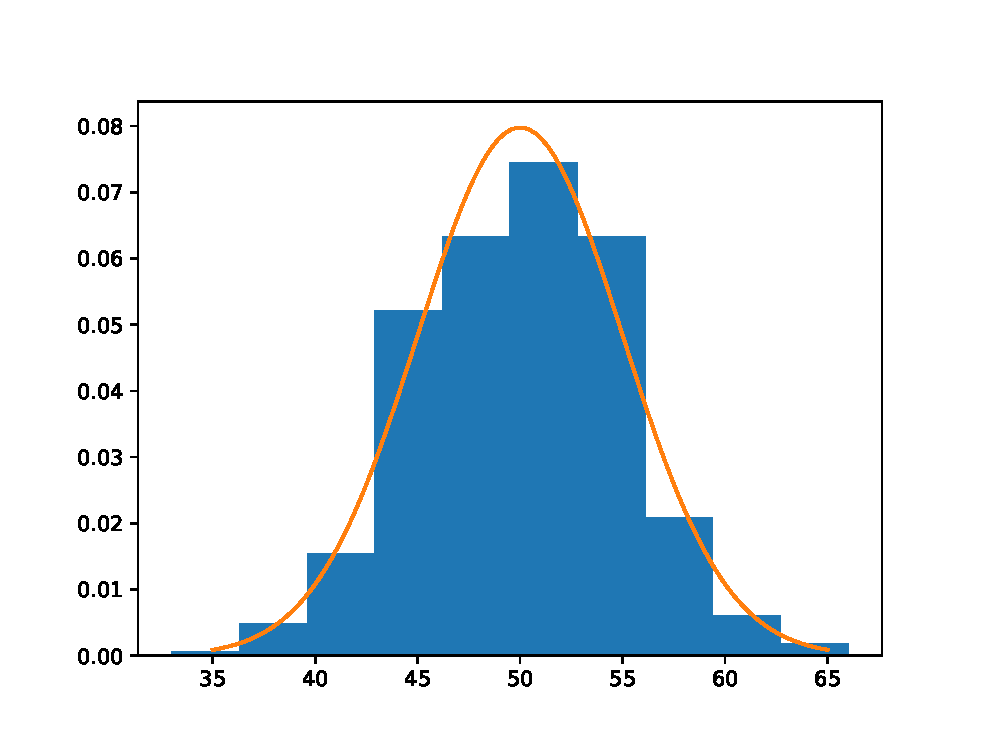
\includegraphics[width=300bp]{wind_si}
\vspace{-18bp}
\end{center}
\caption[]{\label{fig:wind}\small
Data shown are averages of measurements gathered from
the National Airport web site at one-hour intervals over
a 67-day period.  1-$\sigma$ error bars represent sample
standard deviations.  The data clearly indicate that the
best time for sailing on the Potomac is mid-afternoon.
}
\end{figure}
%------------------------------------------------------------------------------

As you can see in Fig.~\ref{fig:wind}, a \LaTeX\ document
can include EPS graphics.  The author can rescale these
figures from inside the document.

For {\sfb very} useful information about how to design your
figures and documents, see here:
\url{http://www.amazon.com/dp/0133966151}~.

\end{document}
